

\chapter{The "Aime" methods for Tie Points computation}


% Conclusion, on peut sans doute limiter le nombre de point avec ScaleStab
% pour filtrage a priori => genre les 500 les plus stable

%---------------------------------------------
%---------------------------------------------
%---------------------------------------------

\section{Fast recognition}

%---------------------------------------------

\subsection{Motivation}
For each image, we have computed tie points. A tie points is made
of a vector $V \in \RR^n)$ . Typically $V$ is invariant
to the main geometric deformation .  Le  $V_1$ and $V_2$
be two tie points, we note :

\begin{itemize}
   \item  $H_{om}(V_1,V_2) $ the fact that two tie points are homologous;
\end{itemize}

Given $V_1,V_2$, there is of course no no oracle that can indicate if  $H_{om}(V_1,V_2)$,
and classically we want to compute  a fast mathematical function $\Psi $ that indicate if two vector $V_1$ and $V_2$
correspond to the same tie points .  The ideal function would be such :

\begin{itemize}
   \item  $\Psi(V_1,V_2)  \iff H_{om}(V_1,V_2)$
\end{itemize}


Of course this impossible, and we introduce the miss rate  and fall out:

\begin{itemize}
   \item   miss rate , probability of $\Psi=0$ knowing $H_{om}=1$ , we note $p_m$;
   \item   fall out , probability of $\Psi=1$ knowing $H_{om}=0$, we note $p_f$;
\end{itemize}

As we cannot have the ideal function $\Psi $ such as $p_m=0$ and $p_f=0$,
we have to compromise, and depending on the circunstances, the price of the
two error, will not be the same. Typically, in indexation step,  we are especially
interested to have a low $p_f$; converselly in recognition step we are
especially interested to have a low  $p_m$.


\subsection{Bits vector}


\section{Gaussian pyramid}

\subsection{Computing $\sigma_0$}

\label{GP:SIGMA0}

The gaussian pyramid is made from a succession of image at different scale that
result from a gaussian filter. How can we justify it :

\begin {itemize} 
   \item  image $I_k$ must be at resolution  $R_k =  R_0 s ^k$,
   \item if we assimmilat  $I_0$ to a (sum of) gaussian of std dev $\sigma_0$  , $I_k$
         must be (sum of)  gaussian  $\sigma_0 * R_k$ 
   \item so we can write $I_k = I_0 \ast G(\sigma_k)$ with $\sigma_k^2 + \sigma_0^2 = (\sigma_0  R_k)^2$;
\end {itemize} 

To compute the pyramid, we need an estimation of $\sigma_0$. Which is quite natural, if the initial
image is very blured, it a high $R_0$, and the value $R_1-R_0 = (s-1)R_0$ is also high, which require
a high value for gaussian filter.

We need a way to estimate the initial value $\sigma_0$. Also it's quite arbirtrary, the way it is
done in MMVII is :


\begin {itemize} 
   \item  assimilate $I_0$ to a gaussian of  std dev $\sigma_0$;
   \item  suppose $I_0$ is well sampled (nor blurred nor aliased);
   \item we traduce it mathematically by  :
\end {itemize} 

\begin{equation}
    \int_{-\infty}^{+\infty} I_0 |x| = \frac{1}{2}
\end{equation}

Due to symetry , we can replace by integral on $[0,+\infty]$ and supresse absolute value :

\begin{equation}
    \int_{0}^{+\infty} \frac{x}{\sigma_0 \sqrt{2\pi}} e^{-\frac{x^2}{2\sigma_0^2}}  = \frac{1}{4}
\end{equation}

We integrate :

\begin{equation}
      \lbrack  \frac{-\sigma_0}{\sqrt{2\pi}} e^{-\frac{x^2}{2\sigma_0^2}}\rbrack  _{0}^{+\infty}  = \frac{1}{4}
\end{equation}

So :

\begin{equation}
      \sigma_0 = \sqrt{\frac{\pi}{8}} \simeq 0.626
\end{equation}


%----------------------------------------
%  A conserver : equations TIPE Lolo
%-----------------------------------------
\COM{
\begin{equation}
   \delta R = \frac{1}{\sigma} \frac{L}{S} = \frac{1}{\sigma}  \frac{2 \pi a }{ e \; dz} 
\end{equation}

\begin{equation}
   \phi  = \iint \overrightarrow{B} \overrightarrow{dS} 
         = B_M \cos(\omega t) \pi a^2
\end{equation}

\begin{equation}
   e = -\frac{d\phi}{dt}= B_M \omega  \sin(\omega t)  \pi a^2
\end{equation}


\begin{equation}
   d P_J = \frac{e^2}{\delta R}  
         = \frac{ (B_M \omega \pi a^2  \sin(\omega t))^2 \sigma_e dz }{2 \pi a}
\end{equation}


\begin{equation}
   <d P_J> = \frac{B_M^2 \; \omega ^2 \; \pi \; a^3 \; e \; \sigma \; dz}{4}
\end{equation}

\begin{equation}
  <P_J> =  \int_{z=0}^H <d P_J> = \frac{B_M^2 \; \omega ^2  \; \pi \;  a^3  \; e  \; \sigma  \; H}{4}
\end{equation}

\begin{equation}
  dU = \delta ^2 Q_{creee} +  \delta ^2 Q_{recue de l'air}
\end{equation}

\begin{equation}
  C dT = <P_J> dt - g 2\pi aH(T-T_a)
\end{equation}

\begin{equation}
  C = \mu c 2 \pi a e H
\end{equation}


\begin{equation}
  \mu c 2 \pi a e H \frac{dT}{dt} = \frac{B_M \omega^2 \pi a^3 e \sigma H}{4} - g 2 \pi a H (T-T_a)
\end{equation}


\begin{equation}
  \tau  \frac{dT}{dt} + T = T_{\infty}
\end{equation}


\begin{equation}
  \tau  = \frac{\mu  c e}{g}
\end{equation}

\begin{equation}
  T_{\infty} - T_a = \frac{(B_M \omega a)^2 e \sigma}{8g}
\end{equation}
}


%---------------------------------------------
%---------------------------------------------
%---------------------------------------------

\section{Matching by relaxation}

\subsection{Notations}

We have two images $I$ and $J$, and two set of characteristic points
in $I$ and $J$ :

\begin{itemize}
   \item $A_i \in I$ for $i \in [1 \cdots M]$;
   \item $B_j \in J$ for $j \in [1 \cdots N]$;
\end{itemize}

We will note $D_{Im}$ the size of the images, typically the length of the diagonal. It will be useful
when we need to set some geometric thresholds.

For each characteristic point, we have both a vector descriptor and a position in the image.
We note :

\begin{itemize}
   \item $A^v_i , B^v_i$  the vector descriptor,  
         $A^v_i, B^v_j \in \mathbb{R}^K $  were the dimension $K$
         is typically some hundreds; however here we are only interested by the fact  there exist 
         some distance $D^v$ between
         vector such that the lower the distance, the more likely is that points are homologous;
         we note $D^v(A^v_i , B^v_i) = D^v(A_i , B_i) $
   \item  $A^p_i , B^p_i$  the position ("pixels")   in images of $A$ and $B$ , 
         $A^p_i , B^p_i \in \mathbb{R}^2$
\end{itemize}


We suppose that we can convert the distance $D^v$ in the likelihood $L$ expressing  that $A$ and $B$
are homologous. For example we  use a threshold $\sigma_v$ and set :

\begin{equation}
    L(A_i,B_j) =  e^{-\frac{D^v(A_i,B_i)}{\sigma_v}} \label{EQ:LikL}
\end{equation}

The transformation from  $D^v$ to $L$  , or even the computation of $\sigma_v$
admitting of formula like \ref{EQ:LikL}, may be an issue. By the way we will admit from
now that we have the function $ L$ , probably a way to rationalize this fact
would be to "learn" it from statistic of "real" homologous points.


\subsection{Formulation}

We want to compute a matching between $A_i$ and $B_j$ that use both the "radiometric context" informations 
and the "spatial consistency" information :

\begin{itemize}
   \item radiometric context : $A_i , B_j$  are matched if, as much as possible, $L(A_i,B_j)$ is high;
   \item spatial consistency : if $A_i$ and $B_j$ are matched, then for each $A'_i$ and $B'_j$ such that ,
         $A'^p_i$ is close to $A^p_i$ and $B'^p_i$ is close to $B^p_i$ , then the likelihood
         to match $A'_i$ and $B'_j$ is higher (i.e. neighbors of my homologous are homologous of
         my neighbors);
\end{itemize}

The principle of relaxation is to compute a non-unique weighted matching and to use
the two pieces of information to iteratively re-compute new value of the weighting. Generally, at
the beginning, the "brute" information (=radiometric context) has a higher importance, and as we go
further we give more importance to relational information (=spatial consistency).

To formalize the problem we consider that we want to compute simultaneously two functions :


\begin{itemize}
   \item a discrete matching function $\psi$  such that $\psi (A_i)$ is the homologous
         of $A_i$, with possibly $\psi (A_i) = 0$  when no match is found for $A_i$,
         and we set  $L(A_i,0) = L_0$ where $L_0$ is a constant;
   \item a geometric \emph{smooth} function $\phi$ .
\end{itemize}

And the criterion on $\psi$ and $\phi$ are to  maximize global
likelihood $\mathcal L(\psi)$ (\ref{Crit:Psi})  while minimizing the
spatial incoherence $ \mathcal S(\psi,\phi)$  (\ref{Crit:PhiPsi}).


\begin{equation}
    \mathcal L(\psi) = \sum  L(A_i,\psi(A_i)) \label{Crit:Psi}
\end{equation}


\begin{equation}
    \mathcal S(\psi,\phi) = \sum  | \psi(A_i)^p - \phi(A^p_i) | \label{Crit:PhiPsi}
\end{equation}

Of course, there must be some strong regularity constraint on $\phi$ so that the
equation ~\ref{Crit:PhiPsi} is not trivial. Generally it belongs to a parametric
space of low dimension (such as similitude, homography ...).


\subsection{Simultaneous $\psi$ and $\phi$ ?}

In most general case, it is quite complicated to compute simultaneously $\psi$
and $\phi$.

\subsubsection{Classical approach}
In the most current case in photogrammetry, a first estimation $\psi_0$ is computed with a simple
strategy as :

\begin{equation}
    \psi_0(A_i) =  \underset{B_j \in J}{\operatorname{argmax}}  L(A_i,B_j) \label{ArgMax:Psi}
\end{equation}

And then $\phi$
is computed to remove false match detected as "outliers" of tested $\phi$. 
There is many tricks to have better result (like symmetric matching), but basically
this is the idea.

A particular and very common case of this simultaneous computation is the case
where $\phi$ represents epipolar geometry and is computed by Ransac. By the way in this
case, the  use of Ransac supposes that we know $\psi$ and that it contains a reasonable
proportion of false matches (typically no more than $50\%$). This case is quite common
for example with images acquired the same time (no diachronism) and tie-points resulting
from SIFT.

\subsubsection{Approach by computing $\phi$ first}

In the problem we want to tackle here, the proportion of false match we would get with
equations like~\ref{ArgMax:Psi} is much too high . So we suppose that we can first
have an \emph{approximate} value $\phi_0$ of $\phi$. We will discuss just after how we can
estimate $\phi_0$.

We have to specify that what we mean by $\phi_0$ is an approximation of $\phi$.
To understand equation~\ref{Phi0:ApproxG}  and~\label{Phi0:Appro} we must
imagine a possible scenario for $\phi$ and $\phi_0$. Typicaly $\phi$, the real
correspondence, will the combination of epipolar geometry and $3D$ scene, so according
to the scene, the $\phi$ can be  continuous or only piece-wise continuous. For $\phi_0$,
in our context it will be a function with few parameters, typically a similitude
plane computed from few points (at least $2$). 

We then formalize "$\phi_0$ approximating  $\phi$" by (see also Fig.~\ref{fig:spatial-consist}) :


\begin{equation}
     | \phi_0(A)  - \phi(A) |  < D_A  \label{Phi0:Appro}
\end{equation}

\begin{equation}
     | (\phi_0(A) - \phi_0(A')) -(\phi(A) - \phi(A')) |  < D_g +  \alpha |A-A'|  \label{Phi0:ApproxG}
\end{equation}

By extension, using equation \ref{Crit:PhiPsi} and criterion $\mathcal S$ we want to minimize,
we will set :

\begin{equation}
     | \phi_0(A)  - \psi(A) |  < D_A  \label{PsiPhi0:Appro}
\end{equation}

\begin{equation}
     | (\phi_0(A) - \phi_0(A')) -(\psi(A) - \psi(A')) |  < D_g +  \alpha |A-A'|  \label{PsiPhi0:ApproxG}
\end{equation}

\begin{figure}
\centering
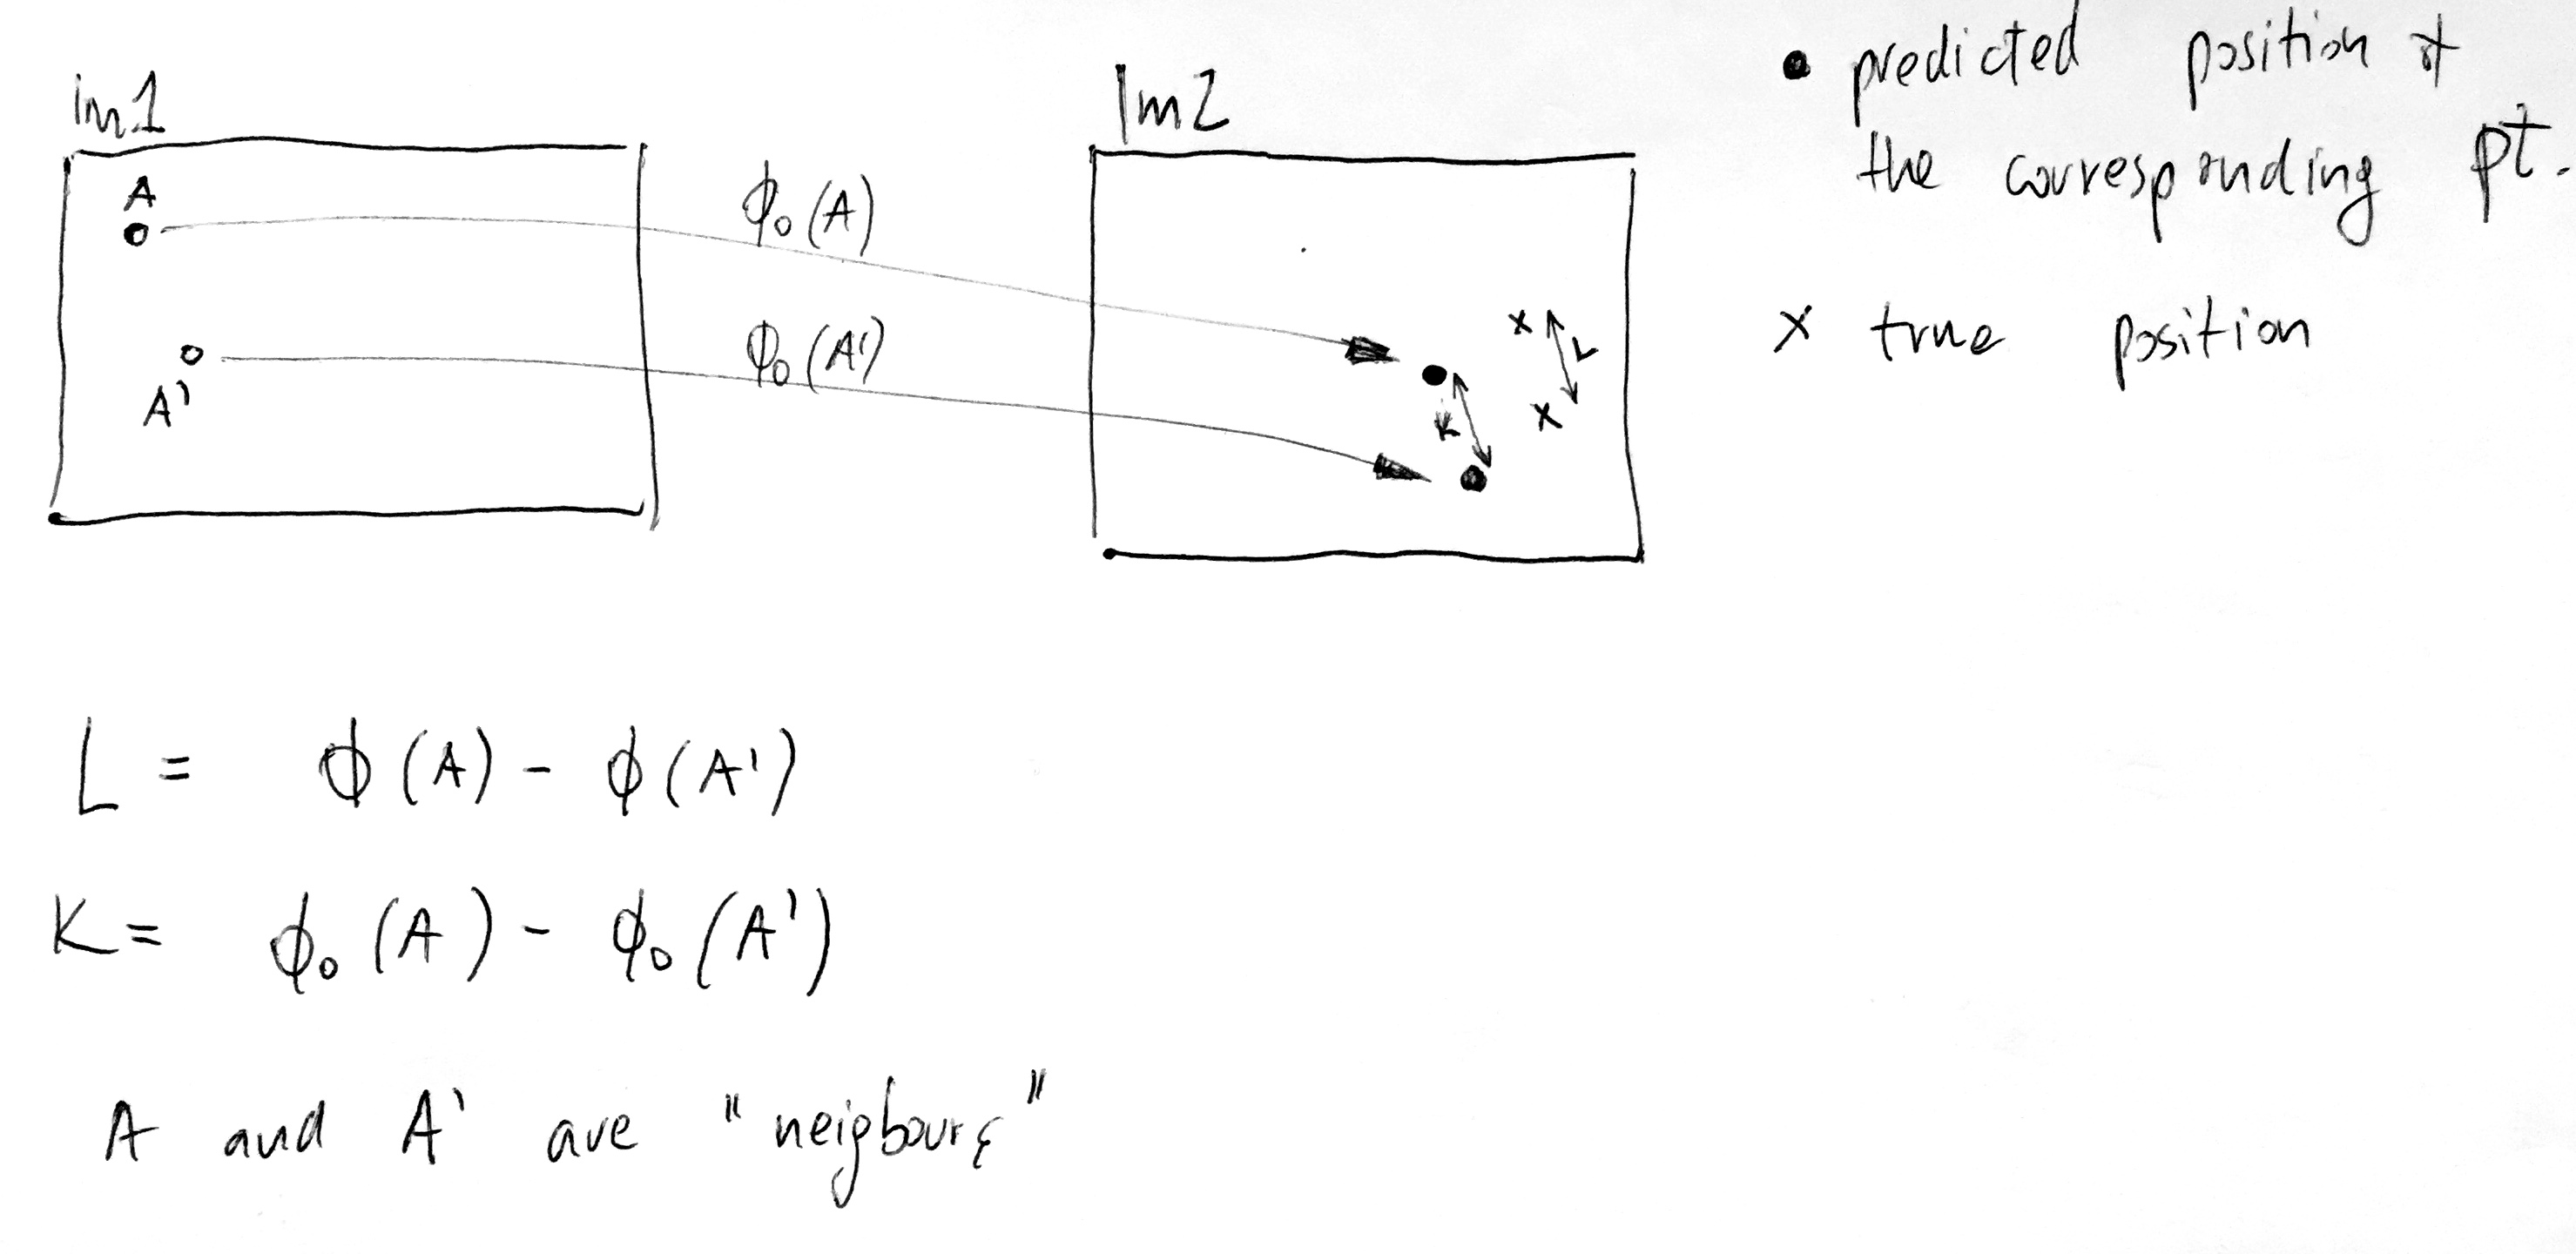
\includegraphics[width=12cm]{Methods/Images/spatial_consist.JPG}\caption{Illustration of equation~\ref{Phi0:ApproxG}.}\label{fig:spatial-consist}
\end{figure}

Let comment these equations  :

\begin{itemize}
   \item in equations~\ref{Phi0:Appro},~\ref{PsiPhi0:Appro},~\ref{PsiPhi0Im:Appro} the value 
         $D_A$ can be relatively high as $\phi0$
         is extracted with few points and the model (similitude) is a rough approximation
         of the "real" model; it seems natural to have $D_A$ proportional to  $D_{Im}$
        (see~\ref{PsiPhi0Im:Appro});

   \item equation~\ref{Phi0:ApproxG},~\ref{PsiPhi0:ApproxG} model the fact that once 
         we "know" that  $ \psi(A)=B$ then $\phi_0$ is a relatively accurate approximation
         of $\psi$ around $A$;  when  $\phi$  is continuous, we don't need $D_g$, however
         when the $3D$ scene is discontinuous, it create discontinuities ; 
         it seems also natural to have $D_g$ proportional to  $D_{Im}$, and obviously
         $D_g$ significantly smaller than $D_A$ (see~\ref{Phi0Im:ApproxG} )
\end{itemize}

So we can write :


\begin{equation}
     | \phi_0(A)  - \psi(A) |  < \beta_A D_{Im}  \label{PsiPhi0Im:Appro}
\end{equation}

\begin{equation}
     | (\phi_0(A) - \phi_0(A')) -(\psi(A) - \psi(A')) |  < \beta_g D_{Im} +  \alpha |A-A'|  \label{Phi0Im:ApproxG}
\end{equation}

Of course, practically, an important question is the values of thresholds $\beta_A, \beta_g, \alpha $.
As a rule of thumb, values of these parameter can be fixed in the following interval :

\begin{itemize}
   \item  $\beta_A \in [0.05,0.2]$, less than $0.05$ would be very optimistic , and by the way this low
          value is probably already sufficient for basic approach like in~\ref{Basic:ArgMax};
          more than $0.2$ would be very pessimistic and by the way difficult to use;

   \item  similarly $\beta_g \in [0.01,0.05]$ and $\alpha \in [0.05,0.3]$
\end{itemize}


And in a first try I woud use $\beta_A=0.1 \;  \beta_g=0.025 \; \alpha=0.15$.


\subsection{Estimation of $\phi_0$}

Obviously, if we cannot estimate $\phi_0$, the previous stuff is useless.
Basically, we can imagine $3$ way to estimate $\phi_0$ :

\begin{itemize}
   \item  the most trivial way is to have an "external" estimation, this can come from
          meta data ("tableau d'assemblage") or from operator measurements (operator select
          manualy two real homologous point and it is sufficient to estimate a similitude);

   \item  another easy way is to use tradional Ransac on a solution like ~\ref{ArgMax:Psi}; 
          with D2Net executed at full resolution, it will probably not work as the proportion
          of false match can be very high; however it is possible to run D2Net at a very low
          resolution, where~\ref{ArgMax:Psi} works not so bad, the accuracy is not so good, but
          it is probably not a problem;

   \item  a third, more sophisticated way, consist to use a non-unique matching at high
          or medium resolution; it is described bellow .
\end{itemize}

Non-unique matching :
\begin{itemize}
   \item  for each point in one image select a number $p$ of its potential matches in the other images, in other words for each point in  $A_i$, select 
            $\Psi (A_i) $ which contains the  $B_j$ corresponding to the $p$
          best scores of $L(A_i,B_j)$; to compute $\Psi$ it is also possible to compute more globally the
          $p * M$ best pairs of all matches $(A_i,B_j)$ where $M$ is a predefined value; here, however, there might be a case where certain points are not assigned a match; to assure that all points have matches a mix of
          both approaches can be adopted (computing a global set of pairs, and also assure to have a minimal
          number of matches per point);

   \item generate solutions, by random selection, if we decide to use similitude,
         it is sufficient to use $2$ pairs of $(A_i,B_j)$  ;  it is also possible to make a biased
         random selection that favors the set of pair having higher likelihood
         (a way to do that is, for each iteration, to generate a few random pairs, 
          and finally select the the pair corresponding to the best likelihood);

   \item for each $2$ pairs, we compute a similitude $S$  and estimate it cost $C(S)$
         by formula below;

   \item after many iteration, select finaly the $S$ minizing $C(S)$.
         by formula above;

\end{itemize}

\begin{equation}
     C(S) = \sum_i (\underset{B_j \in \Psi(A_i)}{\operatorname{Min}}  c(A_i,B_j,S))
\end{equation}

For $c(A_i,B_j,S)$, different formula can be tested, a basic formula proportional to distances, 
one using a threshold to limit the influence of outliers  : 

\begin{equation}
      c(A_i,B_j,S) = Min(|S(A_i)-B_j|,D_A)
\end{equation}

Or a smoother version :

\begin{equation}
      c(A_i,B_j,S) = \frac{|S(A_i)-B_j|}{|S(A_i)-B_j|+D_A)}
\end{equation}

It is also possible to use the likelihood $L(A_i,B_j)$ and merge it with the geometric term , 
however it is always complicated to mix valures of different kind.


\subsection{Basic usage of $\phi_0$}

The easiest way to use $\phi_0$ is to re-use the basic strategy of 
equation~\ref{ArgMax:Psi} but filtering the result with  equation~\ref{Phi0:Appro}  :


\begin{equation}
   \psi_1(A_i) =  \underset{B_j \in \mathcal D(\phi_0(A_i),D_A)}{\operatorname{argmax}}  L(A_i,B_j) 
\end{equation}

Where  $\mathcal D(\phi_0(A_i),D_A)$ is  the disc of center $\phi_0(A_i)$ and radius $D_A$.

\label{Basic:ArgMax}

\subsection{Relaxation}





